\begin{figure}[!htb]
\centering

\usetikzlibrary{shadows,arrows}
% Define the layers to draw the diagram
\pgfdeclarelayer{background}
\pgfdeclarelayer{foreground}
\pgfsetlayers{background,main,foreground}
 
% Define block styles  
\tikzstyle{materia}=[draw, fill=blue!20, text width=6.0em, text centered,
  minimum height=1.5em,drop shadow]
\tikzstyle{Lab} = [materia, text width=8em, minimum width=10em,
  minimum height=3em, rounded corners, drop shadow]
\tikzstyle{texto} = [above, text width=6em, text centered]
\tikzstyle{linepart} = [draw, thick, color=black!50, -latex', dashed]
\tikzstyle{line} = [draw, thick, color=black!50, -latex']
\tikzstyle{ur}=[draw, text centered, minimum height=0.01em]
 
% Define distances for bordering
\newcommand{\blockdist}{1.3}
\newcommand{\edgedist}{1.5}
\newcommand{\myBlock}[2]{node (p#1) [Lab]{#2}}

% Draw background
\newcommand{\background}[5]{%
  \begin{pgfonlayer}{background}
    % Left-top corner of the background rectangle
    \path (#1.west |- #2.north)+(-0.5,0.5) node (a1) {};
    % Right-bottom corner of the background rectanle
    \path (#3.east |- #4.south)+(+0.5,-0.25) node (a2) {};
    % Draw the background
    \path[fill=yellow!20,rounded corners, draw=black!50, dashed]
      (a1) rectangle (a2);
    \path (a1.east |- a1.south)+(0.8,-0.3) node (u1)[texto]
      {\scriptsize\textit{Unidad #5}};
  \end{pgfonlayer}}

\newcommand{\transreceptor}[3]{%
  \path [linepart] (#1.east) -- node [above]
    {\scriptsize Transreceptor #2} (#3);}

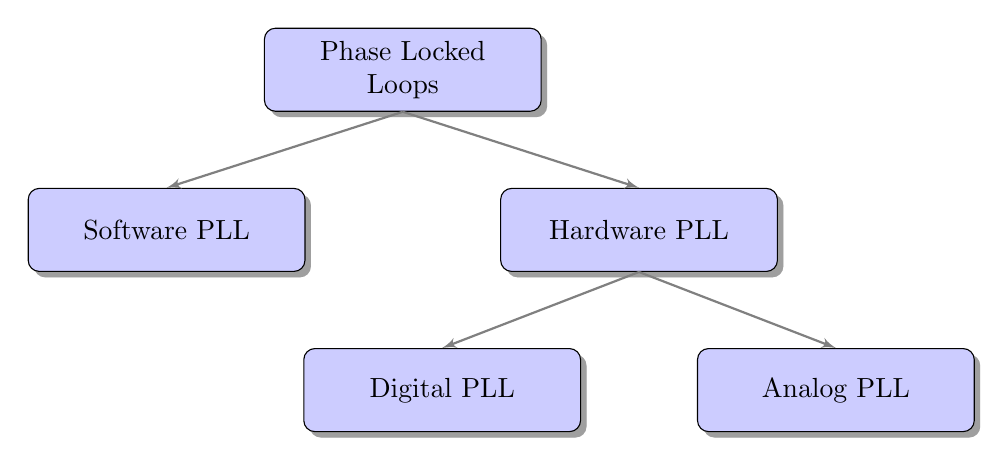
\begin{tikzpicture}[transform shape]
 
 % Draw diagram elements
  \path \myBlock {1}{Phase Locked Loops};
  \path (p1.south)+(-3,-1.5) \myBlock{2}{Software PLL};
  \path (p1.south)+(3,-1.5) \myBlock{3}{Hardware PLL};
  \path (p3.south)+(2.5,-1.5) \myBlock{4}{Analog PLL};
  \path (p3.south)+(-2.5,-1.5) \myBlock{5}{Digital PLL};
     
  % Draw arrows between elements
  \path [line] (p1.south) -- node  {} (p2.north);
  \path [line] (p1.south) -- node  {} (p3.north);
  \path [line] (p3.south) -- node  {} (p4.north);
  \path [line] (p3.south) -- node  {} (p5.north);

\end{tikzpicture}
\caption{Taxonomy}
\label{fig:Taxonomy}
\end{figure}